\documentclass{article}

\usepackage[utf8]{inputenc}
\usepackage[bottom=2cm, top=2cm, left=2cm, right=2cm]{geometry}
\usepackage{verbatim}
\usepackage{tikz}
\usepackage[T1]{fontenc}
\usepackage{bm}
\usepackage{listings}
\usetikzlibrary{chains}

\title{Lista 8 - Filas de Prioridades}
\author{Vinícius Couto Tasso}
\date{}

\begin{document}

\maketitle
   
\tikzset{every tree node/.style={minimum size=2em,draw,circle},
         blank/.style={draw=none},
         edge from parent/.style=
         {draw,edge from parent path={(\tikzparentnode) -- (\tikzchildnode)}},
         level distance=1cm}
         
\begin{enumerate}

\item \textbf{Ilustre as operações \textsc{Heap-Extract-Max} e \textsc{Max-Heap-Insert}($\bm{V,size,10}$), de forma independente, sobre o heap $V = \langle 15, 13, 9, 5, 12, 8, 7, 4, 0, 6, 2, 1 \rangle$ (mostre uma árvore para cada operação).}

\begin{center}
    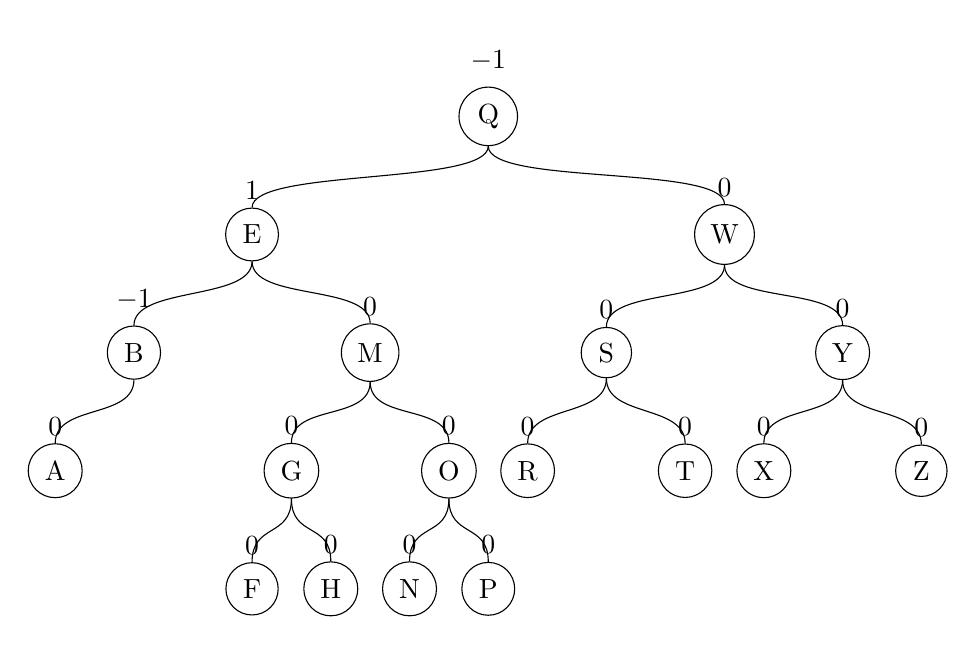
\begin{tikzpicture}[
       edge from parent path=
    {(\tikzparentnode.south) .. controls +(0,-.5) and +(0,.5)
                             .. (\tikzchildnode.north)},
    level 1/.style={sibling distance=6cm},                        
    level 2/.style={sibling distance=3cm},                         
    level 3/.style={sibling distance=2cm},
    level 4/.style={sibling distance=1cm},
   every node/.style={draw,circle},
   label distance=-1mm]
   
\node[label=90:$-1$] {Q}
    child {node[label=90:$1$] {E}
        child {node[label=90:$-1$] {B}
            child {node[label=90:$0$] {A}}
            child[missing]{}
        }
        child {node[label=90:$0$] {M}
            child {node[label=90:$0$] {G}
                child {node[label=90:$0$] {F}}
                child {node[label=90:$0$] {H}}
            }
            child {node[label=90:$0$] {O}
                child {node[label=90:$0$] {N}}
                child {node[label=90:$0$] {P}}
            }
        }
    }   
    child {node[label=90:$0$] {W}
        child {node[label=90:$0$] {S}
            child {node[label=90:$0$] {R}}
            child {node[label=90:$0$] {T}}
            }
        child {node[label=90:$0$] {Y}
            child {node[label=90:$0$] {X}}
            child {node[label=90:$0$] {Z}}
            }
    };

\end{tikzpicture}
\end{center}

\item \textbf{Mostre como implementar uma operação \textsc{Heap-Decrease-Key} para um heap máximo.}

% Remove A

\begin{center}
    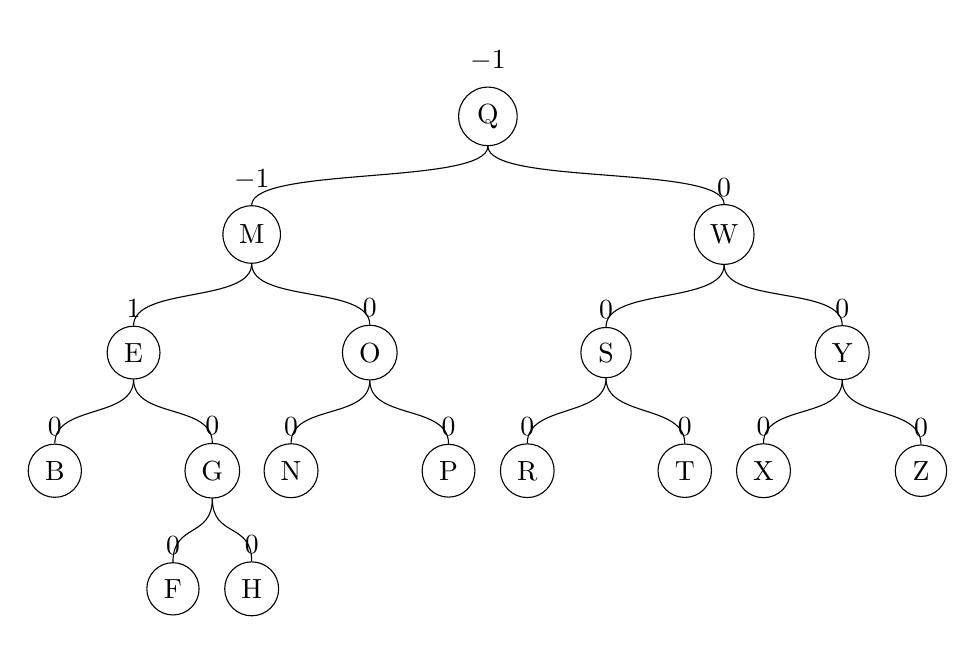
\begin{tikzpicture}[
       edge from parent path=
    {(\tikzparentnode.south) .. controls +(0,-.5) and +(0,.5)
                             .. (\tikzchildnode.north)},
    level 1/.style={sibling distance=6cm},                        
    level 2/.style={sibling distance=3cm},                         
    level 3/.style={sibling distance=2cm},
    level 4/.style={sibling distance=1cm},
   every node/.style={draw,circle},
   label distance=-1mm]
   
\node[label=90:$-1$] {Q}
    child {node[label=90:$-1$] {M}
        child {node[label=90:$1$] {E}
            child {node[label=90:$0$] {B}}
            child {node[label=90:$0$] {G}
                child {node[label=90:$0$] {F}}
                child {node[label=90:$0$] {H}}
            }
        }
        child {node[label=90:$0$] {O}
            child {node[label=90:$0$] {N}}
            child {node[label=90:$0$] {P}}
        }
    }   
    child {node[label=90:$0$] {W}
        child {node[label=90:$0$] {S}
            child {node[label=90:$0$] {R}}
            child {node[label=90:$0$] {T}}
            }
        child {node[label=90:$0$] {Y}
            child {node[label=90:$0$] {X}}
            child {node[label=90:$0$] {Z}}
            }
    };

\end{tikzpicture}
\end{center}

% Remove H

\begin{center}
    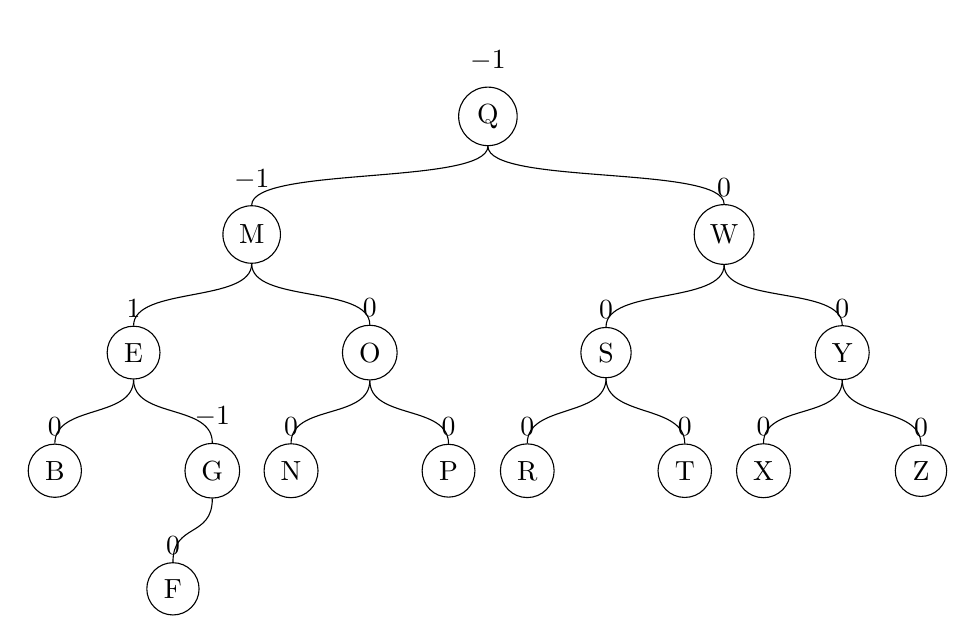
\begin{tikzpicture}[
       edge from parent path=
    {(\tikzparentnode.south) .. controls +(0,-.5) and +(0,.5)
                             .. (\tikzchildnode.north)},
    level 1/.style={sibling distance=6cm},                        
    level 2/.style={sibling distance=3cm},                         
    level 3/.style={sibling distance=2cm},
    level 4/.style={sibling distance=1cm},
   every node/.style={draw,circle},
   label distance=-1mm]
   
\node[label=90:$-1$] {Q}
    child {node[label=90:$-1$] {M}
        child {node[label=90:$1$] {E}
            child {node[label=90:$0$] {B}}
            child {node[label=90:$-1$] {G}
                child {node[label=90:$0$] {F}}
                child[missing]{}
            }
        }
        child {node[label=90:$0$] {O}
            child {node[label=90:$0$] {N}}
            child {node[label=90:$0$] {P}}
        }
    }   
    child {node[label=90:$0$] {W}
        child {node[label=90:$0$] {S}
            child {node[label=90:$0$] {R}}
            child {node[label=90:$0$] {T}}
            }
        child {node[label=90:$0$] {Y}
            child {node[label=90:$0$] {X}}
            child {node[label=90:$0$] {Z}}
            }
    };

\end{tikzpicture}
\end{center}

% Remove E

\begin{center}
    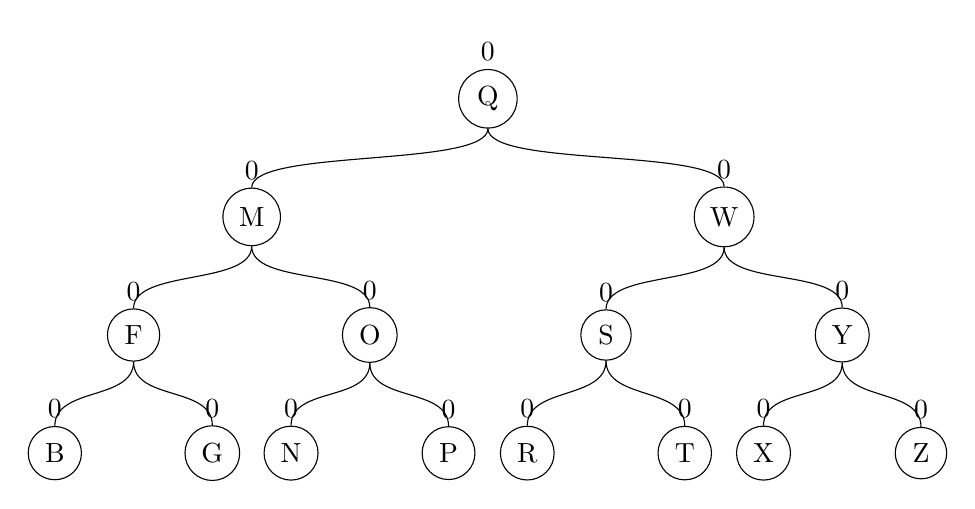
\begin{tikzpicture}[
       edge from parent path=
    {(\tikzparentnode.south) .. controls +(0,-.5) and +(0,.5)
                             .. (\tikzchildnode.north)},
    level 1/.style={sibling distance=6cm},                        
    level 2/.style={sibling distance=3cm},                         
    level 3/.style={sibling distance=2cm},
   every node/.style={draw,circle},
   label distance=-1mm]
   
\node[label=90:$0$] {Q}
    child {node[label=90:$0$] {M}
        child {node[label=90:$0$] {F}
            child {node[label=90:$0$] {B}}
            child {node[label=90:$0$] {G}}
        }
        child {node[label=90:$0$] {O}
            child {node[label=90:$0$] {N}}
            child {node[label=90:$0$] {P}}
        }
    }   
    child {node[label=90:$0$] {W}
        child {node[label=90:$0$] {S}
            child {node[label=90:$0$] {R}}
            child {node[label=90:$0$] {T}}
            }
        child {node[label=90:$0$] {Y}
            child {node[label=90:$0$] {X}}
            child {node[label=90:$0$] {Z}}
            }
    };

\end{tikzpicture}
\end{center}

% Remove W

\begin{center}
    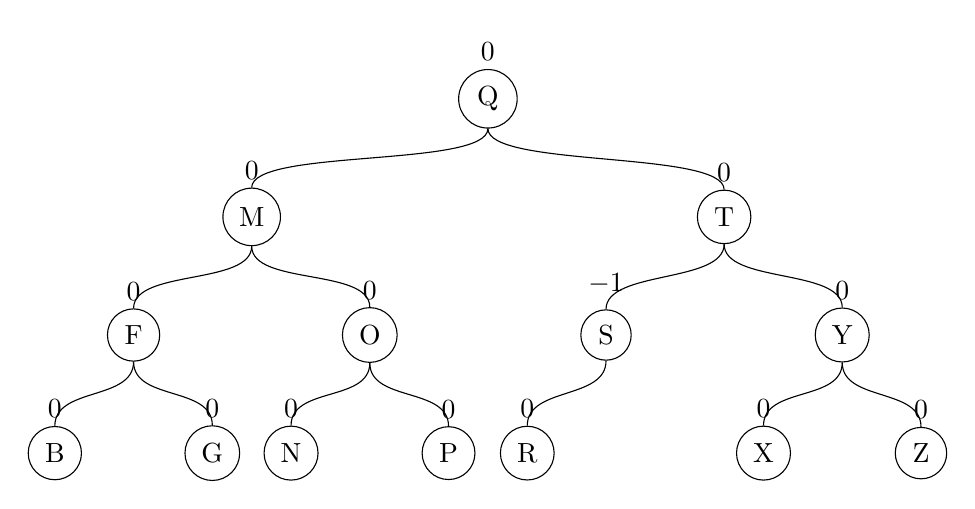
\begin{tikzpicture}[
       edge from parent path=
    {(\tikzparentnode.south) .. controls +(0,-.5) and +(0,.5)
                             .. (\tikzchildnode.north)},
    level 1/.style={sibling distance=6cm},                        
    level 2/.style={sibling distance=3cm},                         
    level 3/.style={sibling distance=2cm},
   every node/.style={draw,circle},
   label distance=-1mm]
   
\node[label=90:$0$] {Q}
    child {node[label=90:$0$] {M}
        child {node[label=90:$0$] {F}
            child {node[label=90:$0$] {B}}
            child {node[label=90:$0$] {G}}
        }
        child {node[label=90:$0$] {O}
            child {node[label=90:$0$] {N}}
            child {node[label=90:$0$] {P}}
        }
    }   
    child {node[label=90:$0$] {T}
        child {node[label=90:$-1$] {S}
            child {node[label=90:$0$] {R}}
            child[missing]{}
            }
        child {node[label=90:$0$] {Y}
            child {node[label=90:$0$] {X}}
            child {node[label=90:$0$] {Z}}
            }
    };

\end{tikzpicture}
\end{center}

% Remove G

\begin{center}
    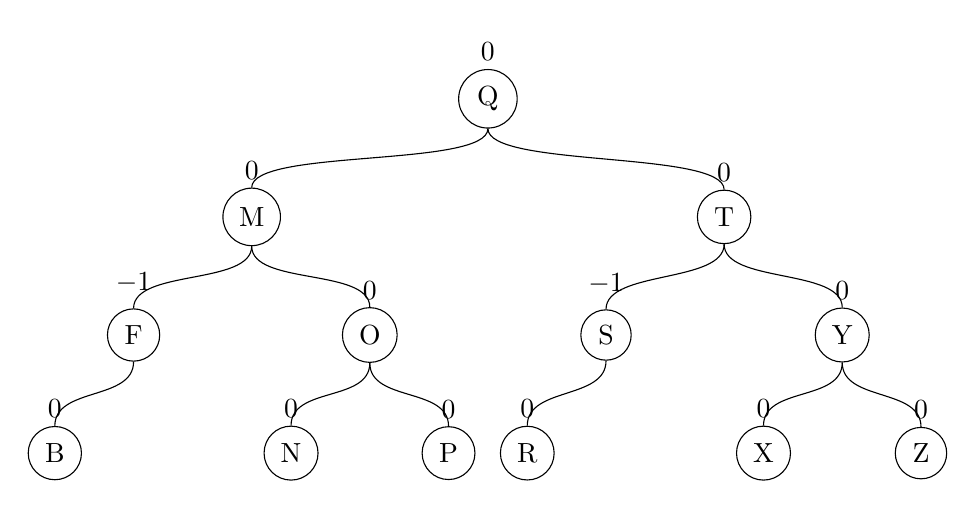
\begin{tikzpicture}[
       edge from parent path=
    {(\tikzparentnode.south) .. controls +(0,-.5) and +(0,.5)
                             .. (\tikzchildnode.north)},
    level 1/.style={sibling distance=6cm},                        
    level 2/.style={sibling distance=3cm},                         
    level 3/.style={sibling distance=2cm},
   every node/.style={draw,circle},
   label distance=-1mm]
   
\node[label=90:$0$] {Q}
    child {node[label=90:$0$] {M}
        child {node[label=90:$-1$] {F}
            child {node[label=90:$0$] {B}}
            child[missing]{}
        }
        child {node[label=90:$0$] {O}
            child {node[label=90:$0$] {N}}
            child {node[label=90:$0$] {P}}
        }
    }   
    child {node[label=90:$0$] {T}
        child {node[label=90:$-1$] {S}
            child {node[label=90:$0$] {R}}
            child[missing]{}
            }
        child {node[label=90:$0$] {Y}
            child {node[label=90:$0$] {X}}
            child {node[label=90:$0$] {Z}}
            }
    };

\end{tikzpicture}
\end{center}

% Remove N

\begin{center}
    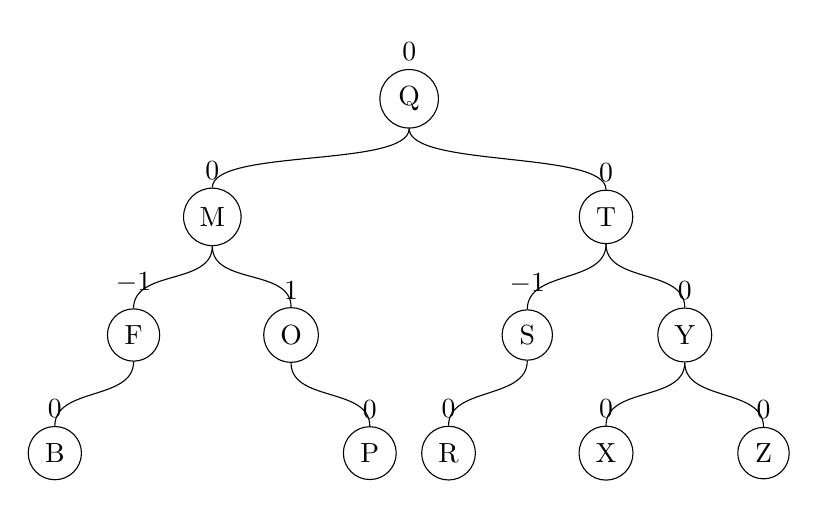
\begin{tikzpicture}[
       edge from parent path=
    {(\tikzparentnode.south) .. controls +(0,-.5) and +(0,.5)
                             .. (\tikzchildnode.north)},
    level 1/.style={sibling distance=5cm},                        
    level 2/.style={sibling distance=2cm},                         
    level 3/.style={sibling distance=2cm},
   every node/.style={draw,circle},
   label distance=-1mm]
   
\node[label=90:$0$] {Q}
    child {node[label=90:$0$] {M}
        child {node[label=90:$-1$] {F}
            child {node[label=90:$0$] {B}}
            child[missing]{}
        }
        child {node[label=90:$1$] {O}
            child[missing]{}
            child {node[label=90:$0$] {P}}
        }
    }   
    child {node[label=90:$0$] {T}
        child {node[label=90:$-1$] {S}
            child {node[label=90:$0$] {R}}
            child[missing]{}
            }
        child {node[label=90:$0$] {Y}
            child {node[label=90:$0$] {X}}
            child {node[label=90:$0$] {Z}}
            }
    };

\end{tikzpicture}
\end{center}

% Remove P

\begin{center}
    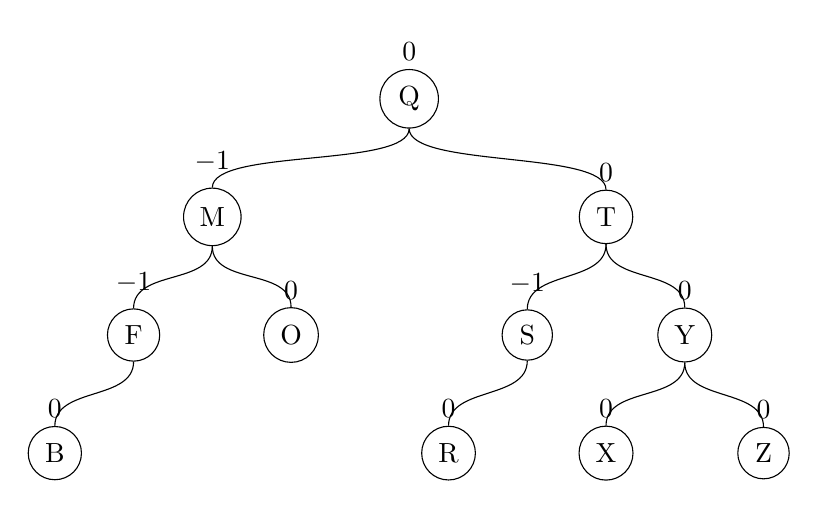
\begin{tikzpicture}[
       edge from parent path=
    {(\tikzparentnode.south) .. controls +(0,-.5) and +(0,.5)
                             .. (\tikzchildnode.north)},
    level 1/.style={sibling distance=5cm},                        
    level 2/.style={sibling distance=2cm},                         
    level 3/.style={sibling distance=2cm},
   every node/.style={draw,circle},
   label distance=-1mm]
   
\node[label=90:$0$] {Q}
    child {node[label=90:$-1$] {M}
        child {node[label=90:$-1$] {F}
            child {node[label=90:$0$] {B}}
            child[missing]{}
        }
        child {node[label=90:$0$] {O}}
    }   
    child {node[label=90:$0$] {T}
        child {node[label=90:$-1$] {S}
            child {node[label=90:$0$] {R}}
            child[missing]{}
            }
        child {node[label=90:$0$] {Y}
            child {node[label=90:$0$] {X}}
            child {node[label=90:$0$] {Z}}
            }
    };

\end{tikzpicture}
\end{center}

% Remove O

\begin{center}
    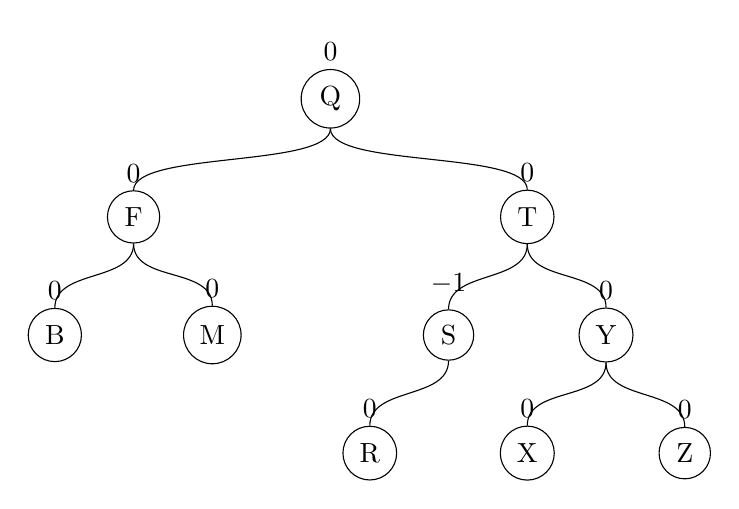
\begin{tikzpicture}[
       edge from parent path=
    {(\tikzparentnode.south) .. controls +(0,-.5) and +(0,.5)
                             .. (\tikzchildnode.north)},
    level 1/.style={sibling distance=5cm},                        
    level 2/.style={sibling distance=2cm},                         
    level 3/.style={sibling distance=2cm},
   every node/.style={draw,circle},
   label distance=-1mm]
   
\node[label=90:$0$] {Q}
    child {node[label=90:$0$] {F}
        child {node[label=90:$0$] {B}}
        child {node[label=90:$0$] {M}}
    }   
    child {node[label=90:$0$] {T}
        child {node[label=90:$-1$] {S}
            child {node[label=90:$0$] {R}}
            child[missing]{}
            }
        child {node[label=90:$0$] {Y}
            child {node[label=90:$0$] {X}}
            child {node[label=90:$0$] {Z}}
            }
    };

\end{tikzpicture}
\end{center}


\end{enumerate}

\end{document}
